% This LaTeX document needs to be compiled with XeLaTeX.
\documentclass[10pt]{article}
\usepackage[utf8]{inputenc}
\usepackage{amsmath}
\usepackage{amsfonts}
\usepackage{amssymb}
\usepackage[version=4]{mhchem}
\usepackage{stmaryrd}
\usepackage{graphicx}
\usepackage[export]{adjustbox}
\graphicspath{ {./images/} }
\usepackage{multirow}
\usepackage[fallback]{xeCJK}
\usepackage{polyglossia}
\usepackage{fontspec}
\setCJKmainfont{Noto Serif CJK TC}

\setmainlanguage{polish}
\setmainfont{CMU Serif}

\title{Egzamin maturalny }

\author{}
\date{}


\begin{document}
\maketitle
CENTRALNA\\
KOMISJA\\
EGZAMINACYJNA\\
WYPEŁNIA ZDAJĄCY

\begin{center}
\begin{tabular}{l}
KOD \\
\begin{tabular}{|l|l|}
\hline
 & PESEL \\
\hline
\end{tabular} \\
\hline
\end{tabular}
\end{center}

\section*{Miejsce na naklejkę.}
Sprawdź, czy kod na naklejce to\\
E-100.

Jeżeli tak - przyklej naklejkę. Jeżeli nie - zgłoś to nauczycielowi.

\section*{MATEMATYKA}
\section*{Poziom podstawowy}
Symbol arkusza\\
EMAP-PO-100-2305

\section*{DATA: 8 maja 2023 r.}
GoDzINA ROZPOCZECCIA: 9:00\\
Czas trWania: 170 minut\\
WYPEŁNIA ZESPÓŁ NADZORUJĄCY\\
Uprawnienia zdającego do: dostosowania zasad oceniania dostosowania w zw. z dyskalkulią nieprzenoszenia zaznaczeń na kartę.

LICZBA PUNKTÓW DO UZYSKANIA: 46

Przed rozpoczęciem pracy z arkuszem egzaminacyjnym

\begin{enumerate}
  \item Sprawdź, czy nauczyciel przekazał Ci właściwy arkusz egzaminacyjny, tj. arkusz we właściwej formule, z właściwego przedmiotu na właściwym poziomie.
  \item Jeżeli przekazano Ci niewłaściwy arkusz - natychmiast zgłoś to nauczycielowi. Nie rozrywaj banderol.
  \item Jeżeli przekazano Ci właściwy arkusz - rozerwij banderole po otrzymaniu takiego polecenia od nauczyciela. Zapoznaj się z instrukcją na stronie 2.
\end{enumerate}

\section*{Instrukcja dla zdającego}
\begin{enumerate}
  \item Sprawdź, czy arkusz egzaminacyjny zawiera 30 stron (zadania 1-36). Ewentualny brak zgłoś przewodniczącemu zespołu nadzorującego egzamin.
  \item Na pierwszej stronie arkusza oraz na karcie odpowiedzi wpisz swój numer PESEL i przyklej naklejkę z kodem.
  \item Odpowiedzi do zadań zamkniętych (1-29) zaznacz na karcie odpowiedzi w części karty przeznaczonej dla zdającego. Zamaluj \(\square\) pola do tego przeznaczone. Błędne zaznaczenie otocz kółkiem ( i zaznacz właściwe.
  \item Pamiętaj, że pominięcie argumentacji lub istotnych obliczeń w rozwiązaniu zadania otwartego (30-36) może spowodować, że za to rozwiązanie nie otrzymasz pełnej liczby punktów.
  \item Rozwiązania zadań i odpowiedzi wpisuj w miejscu na to przeznaczonym.
  \item Pisz czytelnie i używaj tylko długopisu lub pióra z czarnym tuszem lub atramentem.
  \item Nie używaj korektora, a błędne zapisy wyraźnie przekreśl.
  \item Nie wpisuj żadnych znaków w części przeznaczonej dla egzaminatora.
  \item Pamiętaj, że zapisy w brudnopisie nie będą oceniane.
  \item Możesz korzystać z Wybranych wzorów matematycznych, cyrkla i linijki oraz kalkulatora prostego. Upewnij się, czy przekazano Ci broszurę z okładką taką jak widoczna poniżej.\\
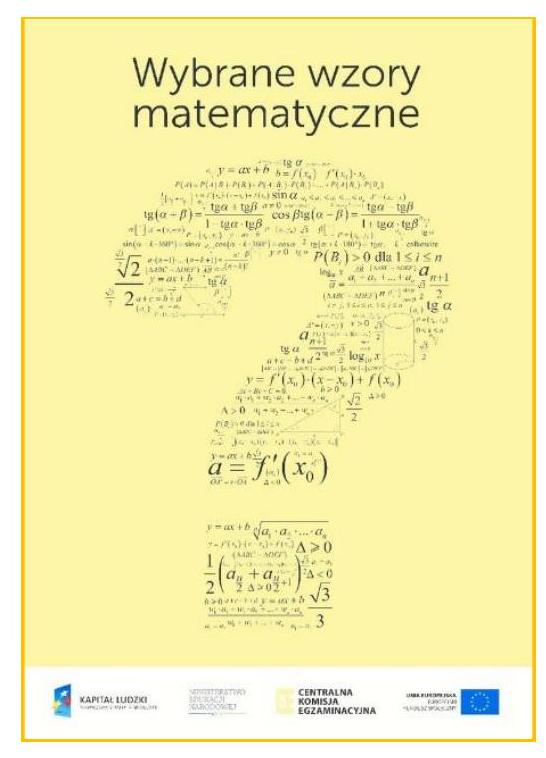
\includegraphics[max width=\textwidth, center]{2024_11_21_cebebd0081c886302305g-02}
\end{enumerate}

\section*{Zadania egzaminacyjne są wydrukowane na następnych stronach.}
W każdym z zadań od 1. do 29. wybierz i zaznacz na karcie odpowiedzi poprawną odpowiedź.

\section*{Zadanie 1. (0-1)}
Liczba \(\log _{9} 27+\log _{9} 3\) jest równa\\
A. 81\\
B. 9\\
C. 4\\
D. 2

\section*{Zadanie 2. (0-1)}
Liczba \(\sqrt[3]{-\frac{27}{16}} \cdot \sqrt[3]{2}\) jest równa\\
A. \(\left(-\frac{3}{2}\right)\)\\
B. \(\frac{3}{2}\)\\
C. \(\frac{2}{3}\)\\
D. \(\left(-\frac{2}{3}\right)\)

\section*{Zadanie 3. (0-1)}
Cenę aparatu fotograficznego obniżono o 15\%, a następnie - o 20\% w odniesieniu do ceny obowiązującej w danym momencie. Po tych dwóch obniżkach aparat kosztuje 340 zł. Przed obiema obniżkami cena tego aparatu była równa\\
A. 500 zt\\
B. 425 zf\\
C. 400 zt\\
D. 375 zf

\section*{Zadanie 4. (0-1)}
Dla każdej liczby rzeczywistej \(a\) wyrażenie \((2 a-3)^{2}-(2 a+3)^{2}\) jest równe\\
A. \(-24 a\)\\
B. 0\\
C. 18\\
D. \(16 a^{2}-24 a\)

\section*{BRUDNOPIS (nie podlega ocenie)}
\begin{center}

\includegraphics[max width=\textwidth]{2024_11_21_cebebd0081c886302305g-05}
\end{center}

Zadanie 5. (0-1)\\
Na rysunku przedstawiono interpretację geometryczną jednego z niżej zapisanych układów równań.\\
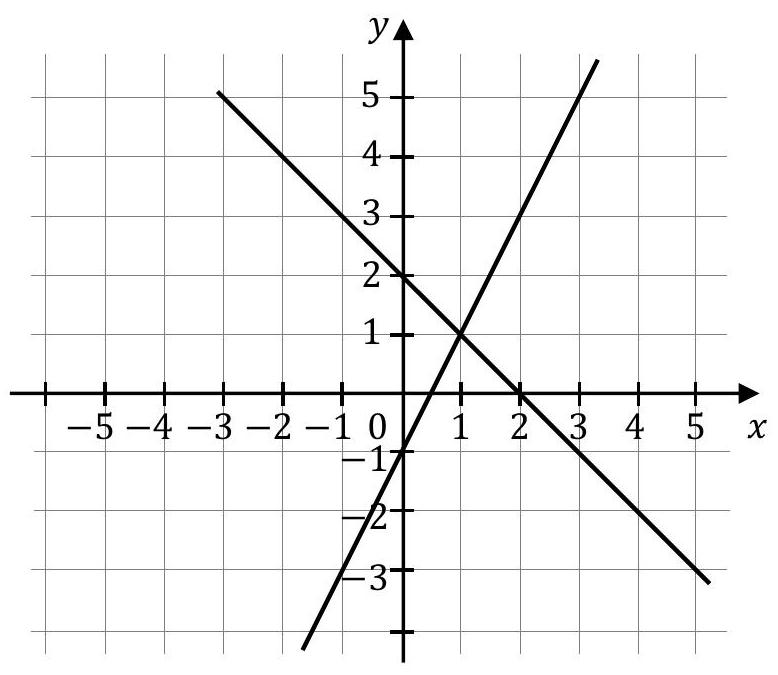
\includegraphics[max width=\textwidth, center]{2024_11_21_cebebd0081c886302305g-06}

Wskaż ten układ równań, którego interpretację geometryczną przedstawiono na rysunku.\\
A. \(\left\{\begin{array}{l}y=-x+2 \\ y=-2 x+1\end{array}\right.\)\\
B. \(\left\{\begin{array}{l}y=x-2 \\ y=-2 x-1\end{array}\right.\)\\
c. \(\left\{\begin{array}{l}y=x-2 \\ y=2 x+1\end{array}\right.\)\\
D. \(\left\{\begin{array}{l}y=-x+2 \\ y=2 x-1\end{array}\right.\)

\section*{Zadanie 6. (0-1)}
Zbiorem wszystkich rozwiązań nierówności

\[
-2(x+3) \leq \frac{2-x}{3}
\]

jest przedział\\
A. \((-\infty,-4)\)\\
B. \((-\infty, 4)\)\\
C. \((-4, \infty)\)\\
D. \((4, \infty)\)

\section*{Zadanie 7. (0-1)}
Jednym z rozwiązań równania \(\sqrt{3}\left(x^{2}-2\right)(x+3)=0\) jest liczba\\
A. 3\\
B. 2\\
C. \(\sqrt{3}\)\\
D. \(\sqrt{2}\)

\section*{BRUDNOPIS (nie podlega ocenie)}
\begin{center}

\includegraphics[max width=\textwidth]{2024_11_21_cebebd0081c886302305g-07}
\end{center}

\section*{Zadanie 8. (0-1)}
Równanie \(\frac{(x+1)(x-1)^{2}}{(x-1)(x+1)^{2}}=0 \mathrm{w}\) zbiorze liczb rzeczywistych\\
A. nie ma rozwiązania.\\
B. ma dokładnie jedno rozwiązanie: -1 .\\
C. ma dokładnie jedno rozwiązanie: 1.\\
D. ma dokładnie dwa rozwiązania: -1 oraz 1 .

\section*{Zadanie 9. (0-1)}
Miejscem zerowym funkcji liniowej \(f(x)=(2 p-1) x+p\) jest liczba \((-4)\). Wtedy\\
A. \(p=\frac{4}{9}\)\\
B. \(p=\frac{4}{7}\)\\
C. \(p=-4\)\\
D. \(p=-\frac{4}{7}\)

\section*{Zadanie 10. (0-1)}
Funkcja liniowa \(f\) jest określona wzorem \(f(x)=a x+b\), gdzie \(a\) i \(b\) są pewnymi liczbami rzeczywistymi. Na rysunku obok przedstawiono fragment wykresu funkcji \(f\) w układzie współrzędnych \((x, y)\).\\
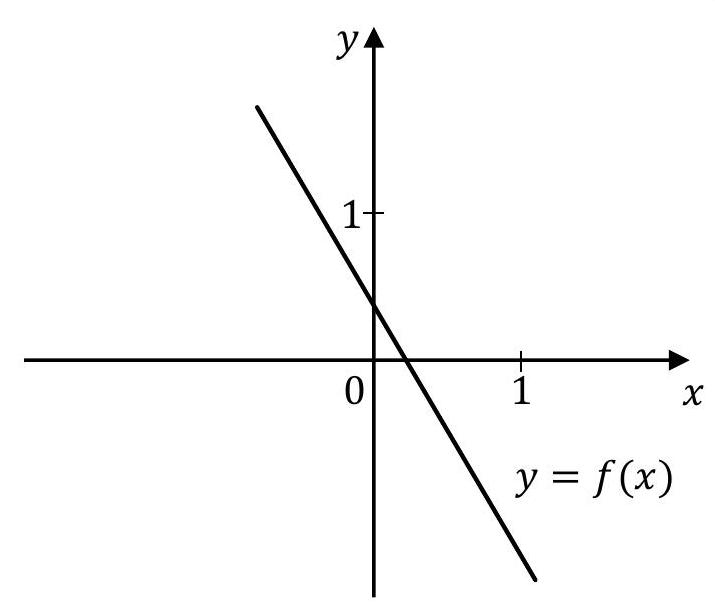
\includegraphics[max width=\textwidth, center]{2024_11_21_cebebd0081c886302305g-08}

Liczba \(a\) oraz liczba \(b\) we wzorze funkcji \(f\) spełniają warunki:\\
A. \(a>0\) i \(b>0\).\\
B. \(a>0\) i \(b<0\).\\
C. \(a<0\) i \(b>0\).\\
D. \(a<0\) i \(b<0\).

\section*{BRUDNOPIS (nie podlega ocenie)}
\begin{center}

\includegraphics[max width=\textwidth]{2024_11_21_cebebd0081c886302305g-09}
\end{center}

\section*{Informacja do zadań 11.-13.}
W układzie współrzędnych \((x, y)\) narysowano wykres funkcji \(y=f(x)\) (zobacz rysunek).\\
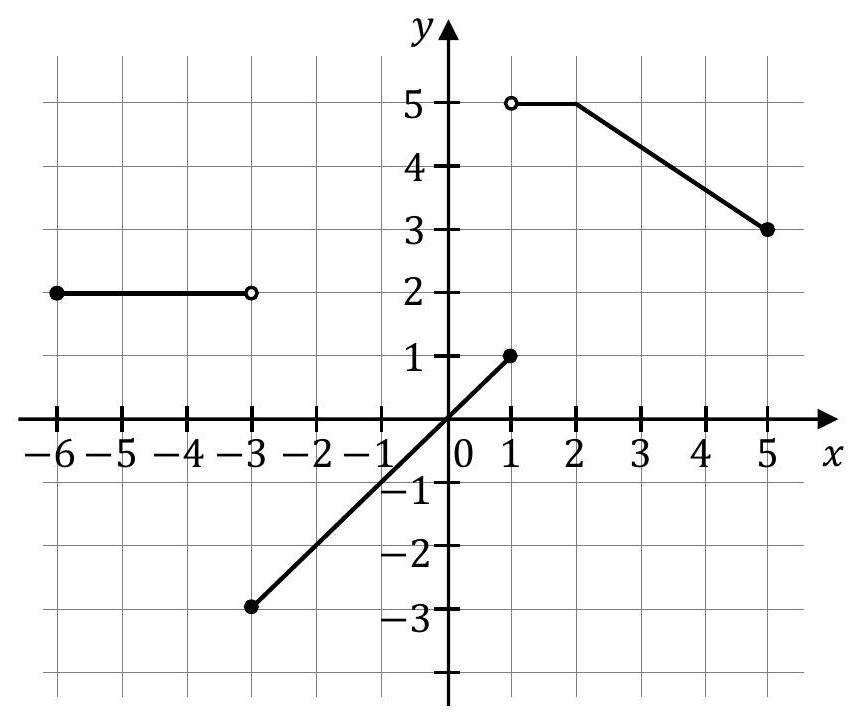
\includegraphics[max width=\textwidth, center]{2024_11_21_cebebd0081c886302305g-10}

Zadanie 11. (0-1)\\
Dziedziną funkcji \(f\) jest zbiór\\
A. \(\langle-6,5\rangle\)\\
B. \((-6,5)\)\\
C. \((-3,5)\)\\
D. \(\langle-3,5\rangle\)

\section*{Zadanie 12. (0-1)}
Funkcja \(f\) jest malejąca w zbiorze\\
A. \((-6,-3)\)\\
B. \(\langle-3,1\rangle\)\\
C. \((1,2)\)\\
D. \(\langle 2,5\rangle\)

\section*{Zadanie 13. (0-1)}
Największa wartość funkcji \(f\) w przedziale \(\langle-4,1\rangle\) jest równa\\
A. 0\\
B. 1\\
C. 2\\
D. 5

\section*{Zadanie 14. (0-1)}
Jednym z miejsc zerowych funkcji kwadratowej \(f\) jest liczba (-5). Pierwsza współrzędna wierzchołka paraboli, będącej wykresem funkcji \(f\), jest równa 3.\\
Drugim miejscem zerowym funkcji \(f\) jest liczba\\
A. 11\\
B. 1\\
C. \((-1)\)\\
D. \((-13)\)

\section*{BRUDNOPIS (nie podlega ocenie)}
\begin{center}

\includegraphics[max width=\textwidth]{2024_11_21_cebebd0081c886302305g-11}
\end{center}

Zadanie 15. (0-1)\\
Ciąg \(\left(a_{n}\right)\) jest określony wzorem \(a_{n}=2^{n} \cdot(n+1)\) dla każdej liczby naturalnej \(n \geq 1\). Wyraz \(a_{4}\) jest równy\\
A. 64\\
B. 40\\
C. 48\\
D. 80

\section*{Zadanie 16. (0-1)}
Trzywyrazowy ciąg (27, 9, \(a-1\) ) jest geometryczny.\\
Liczba a jest równa\\
A. 3\\
B. 0\\
C. 4\\
D. 2

\section*{Zadanie 17. (0-1)}
W układzie współrzędnych zaznaczono kąt \(\alpha\) o wierzchołku w punkcie \(O=(0,0)\). Jedno z ramion tego kąta pokrywa się z dodatnią półosią \(O x\), a drugie przechodzi przez punkt \(P=(-3,1)\) (zobacz rysunek).\\
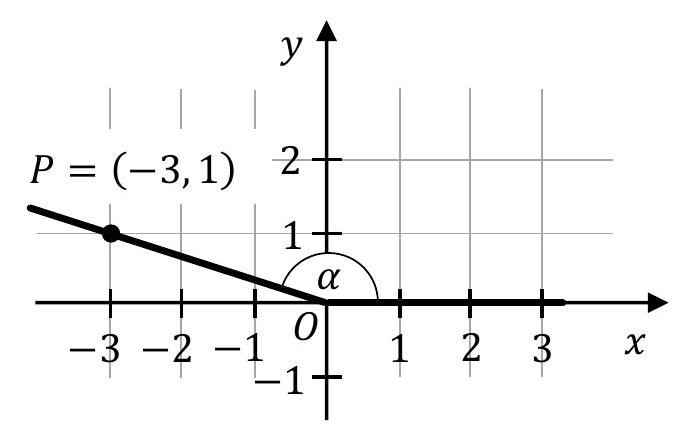
\includegraphics[max width=\textwidth, center]{2024_11_21_cebebd0081c886302305g-12}

Tangens kąta \(\alpha\) jest równy\\
A. \(\frac{1}{\sqrt{10}}\)\\
B. \(\left(-\frac{3}{\sqrt{10}}\right)\)\\
C. \(\left(-\frac{3}{1}\right)\)\\
D. \(\left(-\frac{1}{3}\right)\)

\section*{Zadanie 18. (0-1)}
Dla każdego kąta ostrego \(\alpha\) wyrażenie \(\sin ^{4} \alpha+\sin ^{2} \alpha \cdot \cos ^{2} \alpha\) jest równe\\
A. \(\sin ^{2} \alpha\)\\
B. \(\sin ^{6} \alpha \cdot \cos ^{2} \alpha\)\\
C. \(\sin ^{4} \alpha+1\)\\
D. \(\sin ^{2} \alpha \cdot(\sin \alpha+\cos \alpha) \cdot(\sin \alpha-\cos \alpha)\)

\section*{BRUDNOPIS (nie podlega ocenie)}
\begin{center}

\includegraphics[max width=\textwidth]{2024_11_21_cebebd0081c886302305g-13}
\end{center}

Zadanie 19. (0-1)\\
Punkty \(A, B, C\) leżą na okręgu o środku w punkcie \(O\). Kąt ACO ma miarę \(70^{\circ}\) (zobacz rysunek).\\
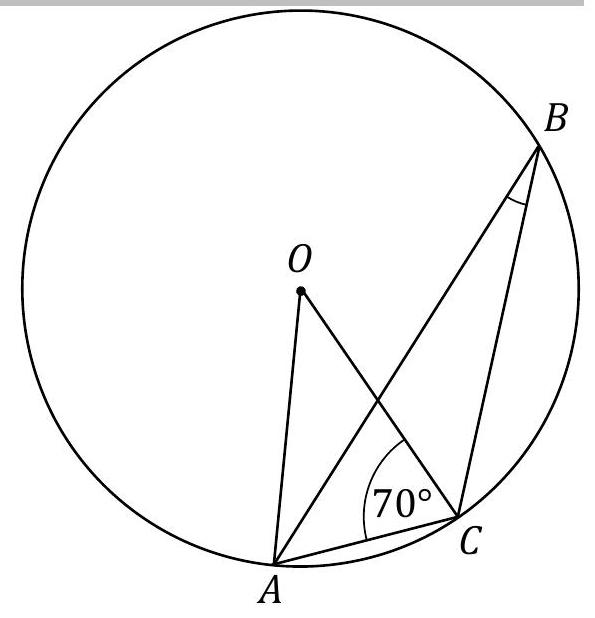
\includegraphics[max width=\textwidth, center]{2024_11_21_cebebd0081c886302305g-14}

Miara kąta ostrego \(A B C\) jest równa\\
A. \(10^{\circ}\)\\
B. \(20^{\circ}\)\\
C. \(35^{\circ}\)\\
D. \(40^{\circ}\)

\section*{Zadanie 20. (0-1)}
W rombie o boku długości \(6 \sqrt{2}\) kąt rozwarty ma miarę \(150^{\circ}\). lloczyn długości przekątnych tego rombu jest równy\\
A. 24\\
B. 72\\
C. 36\\
D. \(36 \sqrt{2}\)

\section*{Zadanie 21. (0-1)}
Przez punkty \(A\) i \(B\), leżące na okręgu o środku \(O\), poprowadzono proste styczne do tego okręgu, przecinające się w punkcie \(C\) (zobacz rysunek).\\
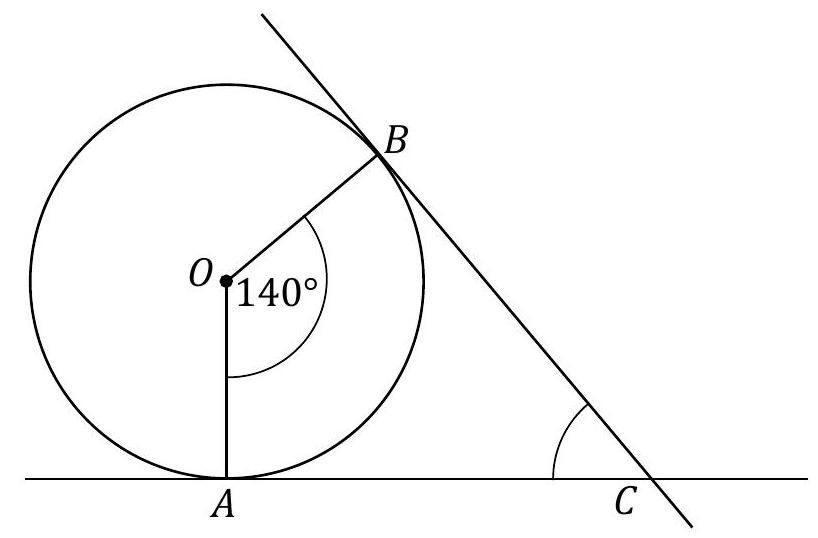
\includegraphics[max width=\textwidth, center]{2024_11_21_cebebd0081c886302305g-14(1)}

Miara kąta \(A C B\) jest równa\\
A. \(20^{\circ}\)\\
B. \(35^{\circ}\)\\
C. \(40^{\circ}\)\\
D. \(70^{\circ}\)

\section*{BRUDNOPIS (nie podlega ocenie)}
\begin{center}

\includegraphics[max width=\textwidth]{2024_11_21_cebebd0081c886302305g-15}
\end{center}

Zadanie 22. (0-1)\\
Dany jest trójkąt \(A B C\), w którym \(|B C|=6\). Miara kąta \(A C B\) jest równa \(150^{\circ}\) (zobacz rysunek).\\
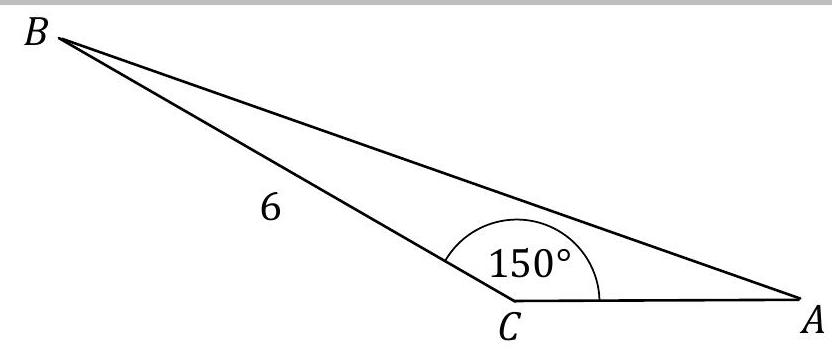
\includegraphics[max width=\textwidth, center]{2024_11_21_cebebd0081c886302305g-16}

Wysokość trójkąta \(A B C\) opuszczona z wierzchołka \(B\) jest równa\\
A. 3\\
B. 4\\
C. \(3 \sqrt{3}\)\\
D. \(4 \sqrt{3}\)

\section*{Zadanie 23. (0-1)}
Dana jest prosta \(k\) o równaniu \(y=-\frac{1}{3} x+2\).\\
Prosta o równaniu \(y=a x+b\) jest równoległa do prostej \(k\) i przechodzi przez punkt \(P=(3,5)\), gdy\\
A. \(a=3\) i \(b=4\).\\
B. \(a=-\frac{1}{3}\) i \(b=4\).\\
C. \(a=3\) i \(b=-4\).\\
D. \(a=-\frac{1}{3}\) i \(b=6\).

\section*{Zadanie 24. (0-1)}
Dane są punkty \(K=(-3,-7)\) oraz \(S=(5,3)\). Punkt \(S\) jest środkiem odcinka \(K L\). Wtedy punkt \(L\) ma współrzędne\\
A. \((13,10)\)\\
B. \((13,13)\)\\
C. \((1,-2)\)\\
D. \((7,-1)\)

\section*{Zadanie 25. (0-1)}
Dana jest prosta o równaniu \(y=2 x-3\). Obrazem tej prostej w symetrii środkowej względem początku układu współrzędnych jest prosta o równaniu\\
A. \(y=2 x+3\)\\
B. \(y=-2 x-3\)\\
C. \(y=-2 x+3\)\\
D. \(y=2 x-3\)

\section*{BRUDNOPIS (nie podlega ocenie)}
\begin{center}

\includegraphics[max width=\textwidth]{2024_11_21_cebebd0081c886302305g-17}
\end{center}

\section*{Zadanie 26. (0-1)}
Dany jest graniastosłup prawidłowy czworokątny, w którym krawędź podstawy ma długość 15. Przekątna graniastosłupa jest nachylona do płaszczyzny podstawy pod kątem \(\alpha\) takim, że \(\cos \alpha=\frac{\sqrt{2}}{3}\).\\
Długość przekątnej tego graniastosłupa jest równa\\
A. \(15 \sqrt{2}\)\\
B. 45\\
C. \(5 \sqrt{2}\)\\
D. 10

\section*{Zadanie 27. (0-1)}
Średnia arytmetyczna liczb \(x, y, z\) jest równa 4.\\
Średnia arytmetyczna czterech liczb: \(1+x, 2+y, 3+z, 14\), jest równa\\
A. 6\\
B. 9\\
C. 8\\
D. 13

\section*{Zadanie 28. (0-1)}
Wszystkich liczb naturalnych pięciocyfrowych, w których zapisie dziesiętnym występują tylko cyfry 0,5,7 (np. 57 075, 55 555), jest\\
A. \(5^{3}\)\\
B. \(2 \cdot 4^{3}\)\\
C. \(2 \cdot 3^{4}\)\\
D. \(3^{5}\)

\section*{Zadanie 29. (0-1)}
W pewnym ostrosłupie prawidłowym stosunek liczby \(W\) wszystkich wierzchołków do liczby \(K\) wszystkich krawędzi jest równy \(\frac{W}{K}=\frac{3}{5}\).\\
Podstawą tego ostrosłupa jest\\
A. kwadrat.\\
B. pięciokąt foremny.\\
C. sześciokąt foremny.\\
D. siedmiokąt foremny.

\section*{BRUDNOPIS (nie podlega ocenie)}
\begin{center}

\includegraphics[max width=\textwidth]{2024_11_21_cebebd0081c886302305g-19}
\end{center}

Zadanie 30. (0-2)\\
Rozwiąż nierówność

\[
x(x-2)>2 x^{2}-3
\]

\begin{center}
\begin{tabular}{|c|c|c|c|c|c|c|c|c|c|c|c|c|c|c|c|c|c|c|c|c|c|c|}
\hline
 &  &  &  &  &  &  &  &  &  &  &  &  &  &  &  &  &  &  &  &  &  &  \\
\hline
 &  &  &  &  &  &  &  &  &  &  &  &  &  &  &  &  &  &  &  &  &  &  \\
\hline
 &  &  &  &  &  &  &  &  &  &  &  &  &  &  &  &  &  &  &  &  &  &  \\
\hline
 &  &  &  &  &  &  &  &  &  &  &  &  &  &  &  &  &  &  &  &  &  &  \\
\hline
 &  &  &  &  &  &  &  &  &  &  &  &  &  &  &  &  &  &  &  &  &  &  \\
\hline
 &  &  &  &  &  &  &  &  &  &  &  &  &  &  &  &  &  &  &  &  &  &  \\
\hline
 &  &  &  &  &  &  &  &  &  &  &  &  &  &  &  &  &  &  &  &  &  &  \\
\hline
 &  &  &  &  &  &  &  &  &  &  &  &  &  &  &  &  &  &  &  &  &  &  \\
\hline
 &  &  &  &  &  &  &  &  &  &  &  &  &  &  &  &  &  &  &  &  &  &  \\
\hline
 &  &  &  &  &  &  &  &  &  &  &  &  &  &  &  &  &  &  &  &  &  &  \\
\hline
 &  &  &  &  &  &  &  &  &  &  &  &  &  &  &  &  &  &  &  &  &  &  \\
\hline
 &  &  &  &  &  &  &  &  &  &  &  &  &  &  &  &  &  &  &  &  &  &  \\
\hline
 &  &  &  &  &  &  &  &  &  &  &  &  &  &  &  &  &  &  &  &  &  &  \\
\hline
 &  &  &  &  &  &  &  &  &  &  &  &  &  &  &  &  &  &  &  &  &  &  \\
\hline
 &  &  &  &  &  &  &  &  &  &  &  &  &  &  &  &  &  &  &  &  &  &  \\
\hline
 &  &  &  &  &  &  &  &  &  &  &  &  &  &  &  &  &  &  &  &  &  &  \\
\hline
 &  &  &  &  &  &  &  &  &  &  &  &  &  &  &  &  &  &  &  &  &  &  \\
\hline
 &  &  &  &  &  &  &  &  &  &  &  &  &  &  &  &  &  &  &  &  &  &  \\
\hline
 &  &  &  &  &  &  &  &  &  &  &  &  &  &  &  &  &  &  &  &  &  &  \\
\hline
 &  &  &  &  &  &  &  &  &  &  &  &  &  &  &  &  &  &  &  &  &  &  \\
\hline
 &  &  &  &  &  &  &  &  &  &  &  &  &  &  &  &  &  &  &  &  &  &  \\
\hline
 &  &  &  &  &  &  &  &  &  &  &  &  &  &  &  &  &  &  &  &  &  &  \\
\hline
 &  &  &  &  &  &  &  &  &  &  &  &  &  &  &  &  &  &  &  &  &  &  \\
\hline
 &  &  &  &  &  &  &  &  &  &  &  &  &  &  &  &  &  &  &  &  &  &  \\
\hline
 &  &  &  &  &  &  &  &  &  &  &  & - &  & 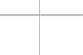
\includegraphics[max width=\textwidth]{2024_11_21_cebebd0081c886302305g-20(1)}
 &  & 
\includegraphics[max width=\textwidth]{2024_11_21_cebebd0081c886302305g-20}
 & 到 &  &  &  &  &  \\
\hline
 &  &  &  &  &  &  &  &  &  &  &  &  &  &  &  &  &  &  &  &  &  &  \\
\hline
 &  &  &  &  &  &  &  &  &  &  &  &  &  &  &  &  &  &  &  &  &  &  \\
\hline
 &  &  &  &  &  &  &  &  &  &  &  &  &  &  &  &  &  &  &  &  &  &  \\
\hline
 &  &  &  &  &  &  &  &  &  &  &  &  &  &  &  &  &  &  &  &  &  &  \\
\hline
 &  &  &  &  &  &  &  &  &  &  &  &  &  &  &  &  &  &  &  &  &  &  \\
\hline
 &  &  &  &  &  &  &  &  &  &  &  &  &  &  &  &  &  &  &  &  &  &  \\
\hline
 &  &  &  &  &  &  &  &  &  &  &  &  &  &  &  &  &  &  &  &  &  &  \\
\hline
 &  &  &  &  &  &  &  &  &  &  &  &  &  &  &  &  &  &  &  &  &  &  \\
\hline
 &  &  &  &  &  &  &  &  &  &  &  &  &  &  &  &  &  &  &  &  &  &  \\
\hline
 &  &  &  &  &  &  &  &  &  &  &  &  &  &  &  &  &  &  &  &  &  &  \\
\hline
 &  &  &  &  &  &  &  &  &  &  &  &  &  &  &  &  &  &  &  &  &  &  \\
\hline
 &  &  &  &  &  &  &  &  &  &  &  &  &  &  &  &  &  &  &  &  &  &  \\
\hline
 &  &  &  &  &  &  &  &  &  &  &  &  &  &  &  &  &  &  &  &  &  &  \\
\hline
 &  &  &  &  &  &  &  &  &  &  &  &  &  &  &  &  &  &  &  &  &  &  \\
\hline
 &  &  &  &  &  &  &  &  &  &  &  &  &  &  &  &  &  &  &  &  &  &  \\
\hline
 &  &  &  &  &  &  &  &  &  &  &  &  &  &  &  &  &  &  &  &  &  &  \\
\hline
 &  &  &  &  &  &  &  &  &  &  &  &  &  &  &  &  &  &  &  &  &  &  \\
\hline
 &  &  &  &  &  &  &  &  &  &  &  &  &  &  &  &  &  &  &  &  &  &  \\
\hline
\end{tabular}
\end{center}

Zadanie 31. (0-2)\\
Pan Stanisław spłacił pożyczkę w wysokości 8910 zł w osiemnastu ratach. Każda kolejna rata była mniejsza od poprzedniej o 30 zł.\\
Oblicz kwotę pierwszej raty.\\

\includegraphics[max width=\textwidth, center]{2024_11_21_cebebd0081c886302305g-21}

\begin{center}
\begin{tabular}{|c|l|c|c|}
\hline
\multirow{2}{*}{\begin{tabular}{c}
Wypełnia \\
egzaminator \\
\end{tabular}} & Nr zadania & 30. & 31. \\
\cline { 2 - 4 }
 & Maks. liczba pkt & 2 & 2 \\
\cline { 2 - 4 }
 & Uzyskana liczba pkt &  &  \\
\hline
\end{tabular}
\end{center}

Zadanie 32. (0-2)\\
Wykaż, że dla każdej liczby rzeczywistej \(x \neq 1\) i dla każdej liczby rzeczywistej \(y\) prawdziwa jest nierówność

\[
x^{2}+y^{2}+5>2 x+4 y
\]

\begin{center}

\includegraphics[max width=\textwidth]{2024_11_21_cebebd0081c886302305g-22}
\end{center}

Zadanie 33. (0-2)\\
Trójkąty prostokątne \(T_{1}\) i \(T_{2}\) są podobne. Przyprostokątne trójkąta \(T_{1}\) mają długości 5 i 12. Przeciwprostokątna trójkąta \(T_{2}\) ma długość 26. Oblicz pole trójkąta \(T_{2}\).\\

\includegraphics[max width=\textwidth, center]{2024_11_21_cebebd0081c886302305g-23}

Zadanie 34. (0-2)\\
W kwadracie \(A B C D\) punkty \(A=(-8,-2)\) oraz \(C=(0,4)\) są końcami przekątnej. Wyznacz równanie prostej zawierającej przekątną \(B D\) tego kwadratu.

\begin{center}
\begin{tabular}{|c|c|c|c|c|c|c|c|c|c|c|c|c|c|c|c|c|c|c|c|c|c|}
\hline
- &  &  &  &  &  &  &  &  &  &  &  &  &  &  &  &  &  &  &  &  &  \\
\hline
 &  &  &  &  &  &  &  &  &  &  &  &  &  &  &  &  &  &  &  &  &  \\
\hline
 &  &  &  &  &  &  &  &  &  &  &  &  &  &  &  &  &  &  &  &  &  \\
\hline
 &  &  &  &  &  &  &  &  &  &  &  &  &  &  &  &  &  &  &  &  &  \\
\hline
 &  &  &  &  &  &  &  &  &  &  &  &  &  &  &  &  &  &  &  &  &  \\
\hline
 &  &  &  &  &  &  &  &  &  &  &  &  &  &  &  &  &  &  &  &  &  \\
\hline
 &  &  &  &  &  &  &  &  &  &  &  &  &  &  &  &  &  &  &  &  &  \\
\hline
 &  &  &  &  &  &  &  &  &  &  &  &  &  &  &  &  &  &  &  &  &  \\
\hline
 &  &  &  &  &  &  &  &  &  &  &  &  &  &  &  &  &  &  &  &  &  \\
\hline
 &  &  &  &  &  &  &  &  &  &  &  &  &  &  &  &  &  &  &  &  &  \\
\hline
 &  &  &  &  &  &  &  &  &  &  &  &  &  &  &  &  &  &  &  &  &  \\
\hline
 &  &  &  &  &  &  &  &  &  &  &  &  &  &  &  &  &  &  &  &  &  \\
\hline
 &  &  &  &  &  &  &  &  &  &  &  &  &  &  &  &  &  &  &  &  &  \\
\hline
 &  &  &  &  &  &  &  &  &  &  &  &  &  &  &  &  &  &  &  &  &  \\
\hline
 &  &  &  &  &  &  &  &  &  &  &  &  &  &  &  &  &  &  &  &  &  \\
\hline
 &  &  &  &  &  &  &  &  &  &  &  &  &  &  &  &  &  &  &  &  &  \\
\hline
 &  &  &  &  &  &  &  &  &  &  &  &  &  &  &  &  &  &  &  &  &  \\
\hline
 &  &  &  &  &  &  &  &  &  &  &  &  &  &  &  &  &  &  &  &  &  \\
\hline
 &  &  &  &  &  &  &  &  &  &  &  &  &  &  &  &  &  &  &  &  &  \\
\hline
 &  &  &  &  &  &  &  &  &  &  &  &  &  &  &  &  &  &  &  &  &  \\
\hline
 &  &  &  &  &  &  &  &  &  &  &  &  &  &  &  &  &  &  &  &  &  \\
\hline
 &  &  &  &  &  &  &  &  &  &  &  &  &  &  &  &  &  &  &  &  &  \\
\hline
 &  &  &  &  &  &  &  &  &  &  &  &  &  &  &  &  &  &  &  &  &  \\
\hline
 &  &  &  &  &  &  &  &  &  &  &  &  &  &  &  &  &  &  &  &  &  \\
\hline
 &  &  &  &  &  &  &  &  &  &  &  &  &  &  &  &  &  &  &  &  &  \\
\hline
 &  &  &  &  &  &  &  &  &  &  &  &  &  &  &  &  &  &  &  &  &  \\
\hline
 &  &  &  &  &  &  &  &  &  &  &  &  &  &  &  &  &  &  &  &  &  \\
\hline
 &  &  &  &  &  &  &  &  &  &  &  &  &  &  &  &  &  &  &  &  &  \\
\hline
 &  &  &  &  &  &  &  &  &  &  &  &  &  &  &  &  &  &  &  &  &  \\
\hline
 &  &  &  &  &  &  &  &  &  &  &  &  &  &  &  &  &  &  &  &  &  \\
\hline
 &  &  &  &  &  &  &  &  &  &  &  &  &  &  &  &  &  &  &  &  &  \\
\hline
 &  &  &  &  &  &  &  &  &  &  &  &  &  &  &  &  &  &  &  &  &  \\
\hline
 &  &  &  &  &  &  &  &  &  &  &  &  &  &  &  &  &  &  &  &  &  \\
\hline
 &  &  &  &  &  &  &  &  &  &  &  &  &  &  &  &  &  &  &  &  &  \\
\hline
 &  &  &  &  &  &  &  &  &  &  &  &  &  &  &  &  &  &  &  &  &  \\
\hline
 &  &  &  &  &  &  &  &  &  &  &  &  &  &  &  &  &  &  &  &  &  \\
\hline
 &  &  &  &  &  &  &  &  &  &  &  &  &  &  &  &  &  &  &  &  &  \\
\hline
 &  &  &  &  &  &  &  &  &  &  &  &  &  &  &  &  &  &  &  &  &  \\
\hline
 &  &  &  &  &  &  &  &  &  &  &  &  &  &  &  &  &  &  &  &  &  \\
\hline
 &  &  &  &  &  &  &  &  &  &  &  &  &  &  &  &  &  &  &  &  &  \\
\hline
 &  &  &  &  &  &  &  &  &  &  &  &  &  &  &  &  &  &  &  &  &  \\
\hline
 &  &  &  &  &  &  &  &  &  &  &  &  &  &  &  &  &  &  &  &  &  \\
\hline
 &  &  &  &  &  &  &  &  &  &  &  &  &  &  &  &  &  &  &  &  &  \\
\hline
 &  &  &  &  &  &  &  &  &  &  &  &  &  &  &  &  &  &  &  &  &  \\
\hline
\end{tabular}
\end{center}

Zadanie 35. (0-2)\\
Ze zbioru ośmiu liczb \(\{2,3,4,5,6,7,8,9\}\) losujemy ze zwracaniem kolejno dwa razy po jednej liczbie.\\
Oblicz prawdopodobieństwo zdarzenia \(A\) polegającego na tym, że iloczyn wylosowanych liczb jest podzielny przez 15.\\

\includegraphics[max width=\textwidth, center]{2024_11_21_cebebd0081c886302305g-25}

Zadanie 36. (0-5)\\
Podstawą graniastosłupa prostego \(A B C D E F\) jest trójkąt równoramienny \(A B C\), w którym \(|A C|=|B C|,|A B|=8\). Wysokość trójkąta \(A B C\), poprowadzona z wierzchołka \(C\), ma długość 3. Przekątna CE ściany bocznej tworzy z krawędzią \(C B\) podstawy \(A B C\) kąt \(60^{\circ}\) (zobacz rysunek).\\
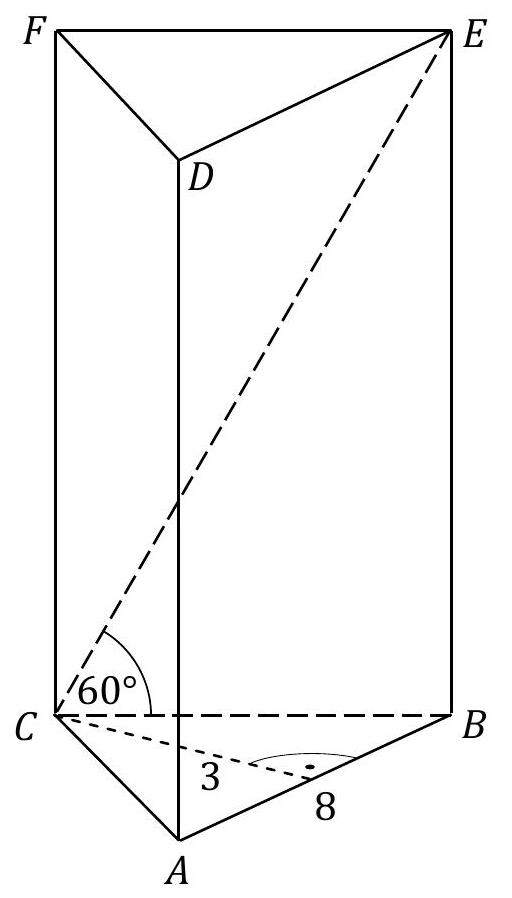
\includegraphics[max width=\textwidth, center]{2024_11_21_cebebd0081c886302305g-26}

Oblicz pole powierzchni całkowitej oraz objętość tego graniastosłupa.\\

\includegraphics[max width=\textwidth, center]{2024_11_21_cebebd0081c886302305g-26(1)}\\

\includegraphics[max width=\textwidth, center]{2024_11_21_cebebd0081c886302305g-27}

\begin{center}
\begin{tabular}{|c|l|c|}
\hline
\multirow{2}{*}{\begin{tabular}{c}
Wypełnia \\
egzaminator \\
\end{tabular}} & Nr zadania & 36. \\
\cline { 2 - 3 }
 & Maks. liczba pkt & 5 \\
\cline { 2 - 3 }
 & Uzyskana liczba pkt &  \\
\hline
\end{tabular}
\end{center}

\section*{BRUDNOPIS (nie podlega ocenie)}

\includegraphics[max width=\textwidth, center]{2024_11_21_cebebd0081c886302305g-28}\\

\includegraphics[max width=\textwidth, center]{2024_11_21_cebebd0081c886302305g-29}\\

\includegraphics[max width=\textwidth, center]{2024_11_21_cebebd0081c886302305g-30}

\section*{MATEMATYKA}
\section*{Poziom podstawowy}
Formuła 2015

\section*{MATEMATYKA}
Poziom podstawowy Formuła 2015

\section*{MATEMATYKA}
Poziom podstawowy\\
Formula 2015


\end{document}